\documentclass[a4j, 10pt, titlepage]{jsarticle}

\usepackage{izumin}
\usepackage{listings}
\lstset{
    language={Ruby},
    frame=shadowbox,
    numbers=left,
    basicstyle={\small},
    breaklines=true
}
\newcommand{\sref}[1]{\lstlistingname ~~\ref{src:#1}}
\begin{document}

\title{数値計算法 課題}
\author{ME1301 泉 将之}
\date{\today}
\maketitle

\ol{[{[}1{]}]
% ================================================================

\li
\eref{q1}(初期条件:\eref{q1-i})をEuler法,Heunの矩形公式,
4次のRunge-Kutta法を用いて解き,厳密解と比較したグラフを書け.
さらに,刻み幅を変化させた時のこれらの数値解の$t = 10$における
誤差(絶対値)の変化を表すグラフを描け.

\eqn{\dd{x}{t} = (\cos t) x (2 - x) \label{eq:q1}}
\eqn{x(0) = 1 \label{eq:q1-i}}

\ol{[(1)]
    \li グラフで厳密解との比較を行う葉には$0 \leq t \leq 10$,
        刻み幅は$h = 0.2$とする.
    \li 誤差の変化を調べる際の刻み幅は
        $0.2 \times 2^{-n} ~~(n = 0, 1, 2, \cdots 9)$とし,
        結果を両対数グラフで表示する.
}

\section*{プログラムリスト}
\sref{ivps},\sref{calcmethod},\sref{q1}に使用したプログラムの
コードを示す.
なお,本稿ではプログラミング言語はRubyを使用する.
InitialValueProblemSolverクラスが常微分方程式の数値解を求めるためのクラスである.
calc\_method.rbに定義されている3つのProcオブジェクトがEuler法,Heunの矩形公式,4次のRunge-Kutta法それぞれの漸化式を表す.
q1.rb内でこれらに定義されたメソッドを順次実行していくことで常微分方程式の数値解を計算する.
Euler法,Heunの矩形公式,4次のRunge-Kutta法はいずれも
漸化式から値を計算していくという共通点がある.
その点に着目し,実装の手間を省くためGoFのデザインパターンの
一つであるStrategyパターンを採用した.
漸化式をConcreateStrategyとし,
インスタンス初期化の際に使用するアルゴリズムの決定を行なっている.
\lstinputlisting[label=src:ivps, caption=initial\_value\_problem\_solver.rb]{src/initial_value_problem_solver.rb}
\lstinputlisting[label=src:calcmethod, caption=calc\_method.rb]{src/calc_method.rb}
\lstinputlisting[label=src:q1, caption=q1.rb]{src/q1.rb}

\section*{考察}
各解析手法で得られた数値解と解析解を比較したグラフを\fref{q1-1}に示す・
\fref{q1-1}を見ると,Heunの矩形公式,4次のRunge-Kutta法は解析解から
プロットしたグラフとほぼ同じ位置に同じ形状のグラフがプロットされた.
一方,Euler法は形状こそ類似しているが位置が少しずれている.
\fig{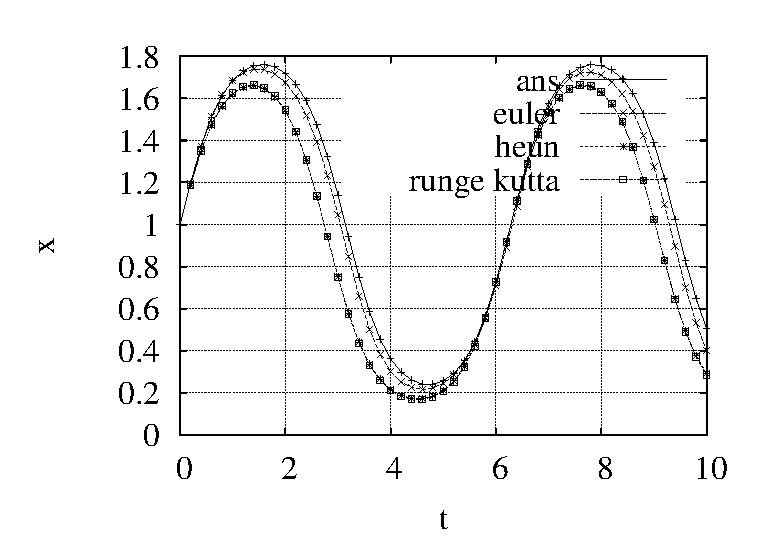
\includegraphics[width=120mm]{img/q1-1.eps}}{Euler法,Heunの矩形公式,4次Runge-Kutta法の厳密解との比較}{q1-1}

各解析手法において,刻み幅を$0.2 \times 2^{-n} ~~(n = 0, 1, 2, \cdots 9)$と変化させた時の解析解との誤差を比較したグラフを\fref{q1-2}に示す.
刻み幅がいずれの値であっても4次のRunge-Kutta法,Heunの矩形公式,Euler法の順に誤差が小さくなっていることがわかる.
また,その誤差は刻み幅が大きくなると減少していくが,その減少幅も4次のRunge-Kutta法,Heunの矩形公式,Euler法の順で大きくなっている.
各手法の精度はEuler法が1次精度,Heunの矩形公式が2次精度,4次のRunge-Kutta法が4次精度である.
よって刻み幅が$\frac{1}{10}$となるとEuler法は誤差が$\frac{1}{10}$,Heunの矩形公式の誤差は$\frac{1}{10^2}$,4次のRunge-Kutta法の誤差は$\frac{1}{10^3}$となっていることがわかる.

\fig{\includegraphics[width=120mm]{img/q1-2.eps}}{Euler法,Heunの矩形公式,4次Runge-Kutta法の厳密解との誤差}{q1-2}


\clearpage
% ================================================================

\li
4次のRunge-Kutta法によって\eref{q2}に示す連立微分方程式の
数値解を求め,そのグラフとLorenz mapを描け.
\eqn{
    \begin{cases}
        \dd{x}{t} &= - \sigma x + \sigma y \\
        \dd{y}{t} &= rx - y - xz \\
        \dd{z}{t} &= -bz + xy
    \end{cases} \label{eq:q2}
}
\eqn{\sigma = 10,~ r = 28,~ b = \frac{8}{3}}
\eqn{x(0) = 0,~ y(0) = 1.1,~ z(0) = 0}

\ol{[(1)]
    \li $0 \leq t \leq 80$とする.滑らかな解が得られるよう適切な
        刻み幅を用いて$(t, z)$,$(x, z)$,$(x, y, z)$の
        グラフを描け.
    \li $z$の極大値を$z_0, z_1, \cdots , z_n, \cdots$とするとき,
        点$(z_n, z_{n+1})$をプロットせよ(Lorenz map).
}

\section*{プログラムリスト}
\sref{q2}に使用したプログラムのソースコードを示す.
前問の\sref{ivps},\sref{calcmethod}を使用する.
InitialValueProblemSolverクラスのインスタンス初期化時にあたえる関数及びその初期値をVectorとして渡すことで連立常微分方程式にも対応可能となっている.
\lstinputlisting[label=src:q2, caption=q2.rb]{src/q2.rb}

\section*{グラフ}

\fig{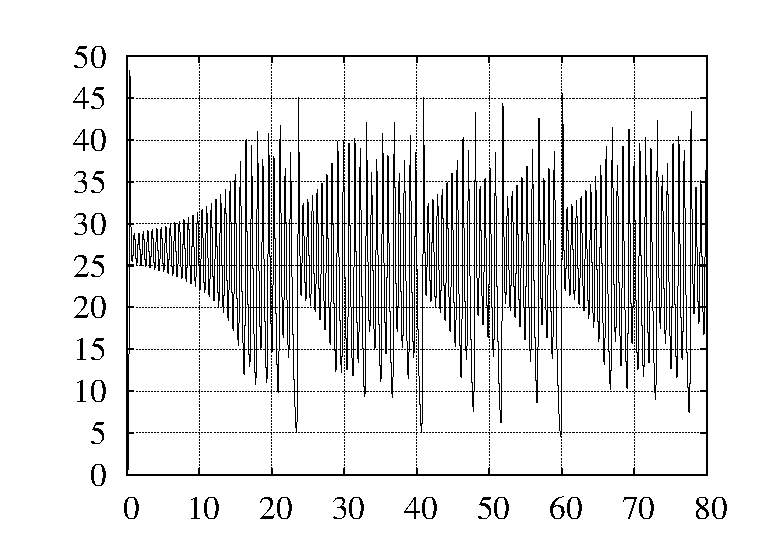
\includegraphics[width=120mm]{img/q2-tz.eps}}{4次Runge-Kutta法による数値解のtz-図}{q2-tz}
\fig{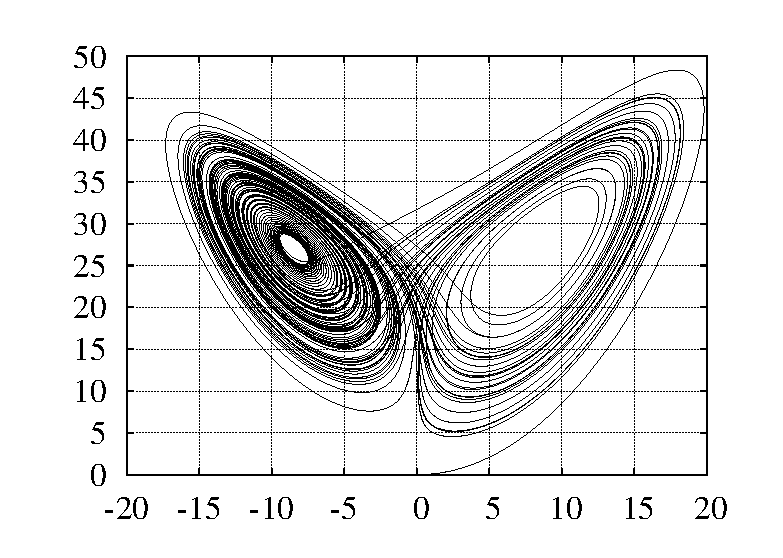
\includegraphics[width=120mm]{img/q2-xz.eps}}{4次Runge-Kutta法による数値解のxz-図}{q2-xz}
\fig{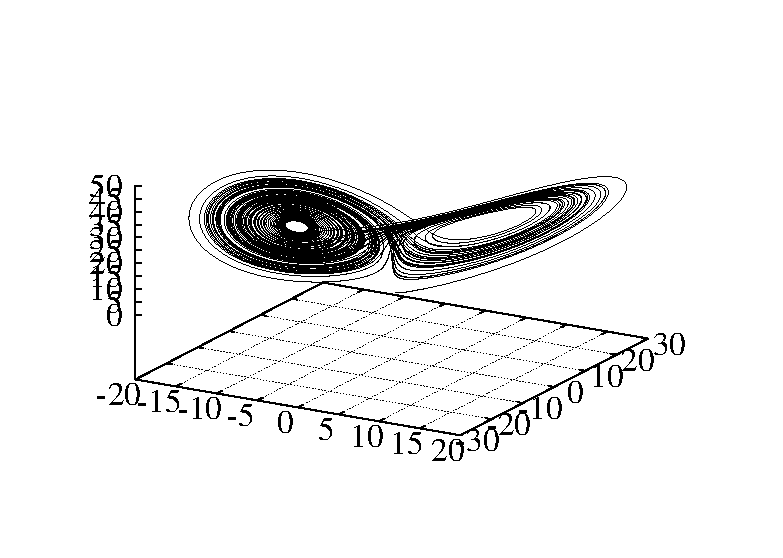
\includegraphics[width=120mm]{img/q2-xyz.eps}}{4次Runge-Kutta法による数値解のxyz-図}{q2-xyz}
\fig{\includegraphics[width=120mm]{img/q2-lorenz_map.eps}}{zの極大値によるLorenz map}{q2-lmap}


\clearpage

% ================================================================

\li
$[-1 ~~ 1]$の一様乱数のみのデータとそれに\eref{q3}を重ねあわせた2種類の
時系列データのパワースペクトルを求め比較考察せよ.

\eqn{
    f(t) =
    \begin{cases}
        \frac{1}{2} (\cos \omega_0 t)^3 & (0 \leq x \leq 2L) \\
        0 & (t < 0,~ t > 2L)
    \end{cases} \label{eq:q3}
}
\eqn{\omega_0 = 5.026548,~ L = 25}

\ol{[(1)]
    \li 離散データの数は$N = 1024$とし,2種類の時系列データと
        パワースペクトルのグラフを描け
}

\section*{ソースコード}
\sref{q3}に使用したプログラムのソースコードを示す.
dftメソッドにサンプリング後の値を与えて離散フーリエ変換をおこない,
power\_spectrumメソッドにdftメソッドの返り値を与えパワースペクトルを導出する.
\lstinputlisting[label=src:q3, caption=q3.rb]{src/q3.rb}

\section*{考察}
一様乱数のみをプロットしたものを\fref{q3-rand},
\eref{q3}と一様乱数を重ねあわせたものを\fref{q3-tf},
そこからパワースペクトルを計算しプロットしたものを\fref{q3-ps}に示す.

\fref{q3-ps}に注目すると$\omega = 64$付近で左右対称となっている
ことがわかる.
\eref{dft}に示す複素フーリエ変換の性質により,その絶対値がサンプルの中央で折り返すためである.
\eqn{
    \hat{F}_{N-k} &= \hat{F_k^*} \notag \\
    \therefore ~~ |\hat{F}_{N-k}| &= |\hat{F_k}| \label{eq:dft}
}

\eref{q3}を式変形すると\eref{cos3}より周波数成分$\omega$と$3\omega$が含まれていることがわかる.
一方,\fref{q3-ps}より最初と2番目のピーク値が出現するときの周波数の値を調べるとそれぞれ$5.026548$,$15.079644$となっている.
これはそれぞれ$\omega_0$,$3\omega_0$の値と等しくなっており,
ここから雑音が含まれていても元のデータに含まれる周波数成分が
取り出せていることがわかる.
以上のことから,一様乱数を重ねあわせた,
即ち雑音が多く含まれたデータでも,離散フーリエ変換を行いパワースペクトルを求めることでもとのデータを抽出できることがわかった.
\eqn{
    \cos^3 \omega_0 t = \frac{1}{4} (3\cos \omega_0 t + \cos 3\omega_0 t)
    \label{eq:cos3}
}
\fig{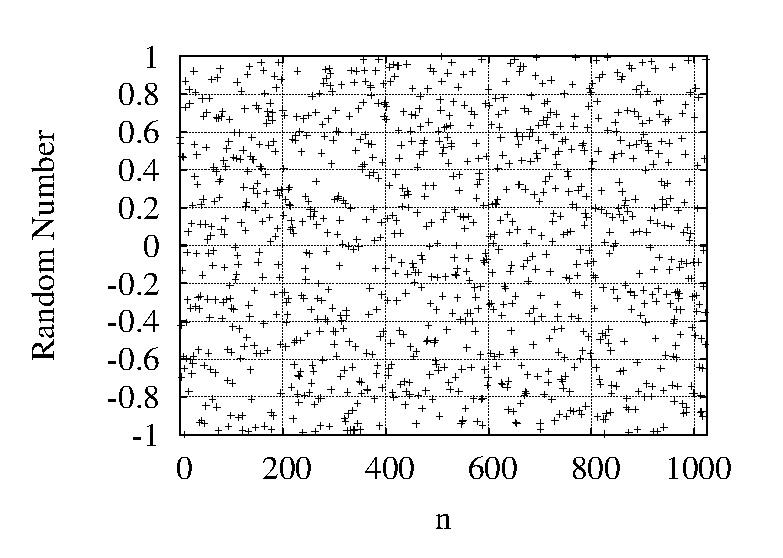
\includegraphics[width=120mm]{img/q3-rand.eps}}{一様乱数}{q3-rand}
\fig{\includegraphics[width=120mm]{img/q3-tf.eps}}{\eref{q3}と一様乱数の重ねあわせ}{q3-tf}
\fig{\includegraphics[width=120mm]{img/q3-ps.eps}}{パワースペクトル図}{q3-ps}
}
\end{document}